\chapter{Implementazione}
In questo capitolo si procede con l'implementazione del nuovo sistema, partendo dai design pattern seguiti per lo sviluppo. Si passa in seguito alla documentazione per definire quali API sono state sviluppate e in che modo sono state suddivise tra i servizi, procedendo con la presentazione dei framework utilizzati per la creazione dei componenti, mostrandone le relative parti di codice. Infine verrà mostrata la struttura del progetto e la sua suddivisione in moduli, e come questi comunicano tra loro.
\label{chap:implementation}

\section{Design Pattern}
\subsection{Inversion of Control}
L'\emph{Inversion of Control (IOC)} è il design pattern su cui si basano la maggior parte dei framework moderni: la sua implementazione è stata quindi indispensabile. Normalmente utilizzando una libreria è il nostro codice a richiamare gli elementi definiti all'interno di essa. Con l'introduzione di questo principio è il nostro codice ad essere richiamato dai componenti del framework, da qui il concetto di \emph{`inversione del controllo'}.

\subsubsection{Façade Pattern}
Questo design pattern contribuisce alla semplificazione delle interazioni con il framework o un set complesso di classi. Quando il codice lavora con un vasto set di oggetti appartenenti a librerie o framework sofisticati, normalmente è necessario inizializzare tali oggetti, tenere traccia delle loro dipendenze e chiamare i relativi metodi nel giusto ordine. In questo modo però il nostro sistema risulta strettamente legato all’implementazione di tali framework rendendolo difficile da mantenere. Il pattern risponde a questo problema. Una Facade è una classe che gestisce al posto nostro la logica appena descritta.

\paragraph{}Utilizziamo uno schema del sito \emph{Refactoring Guru} \cite{refactoring:facadepattern} per semplificare i concetti alla base del suo funzionamento. Prendendo come riferimento la figura [\ref{fig:facadepattern}] presentiamo gli elementi che lo compongono il pattern strutturale:



\begin{figure}[H]
    \centering
    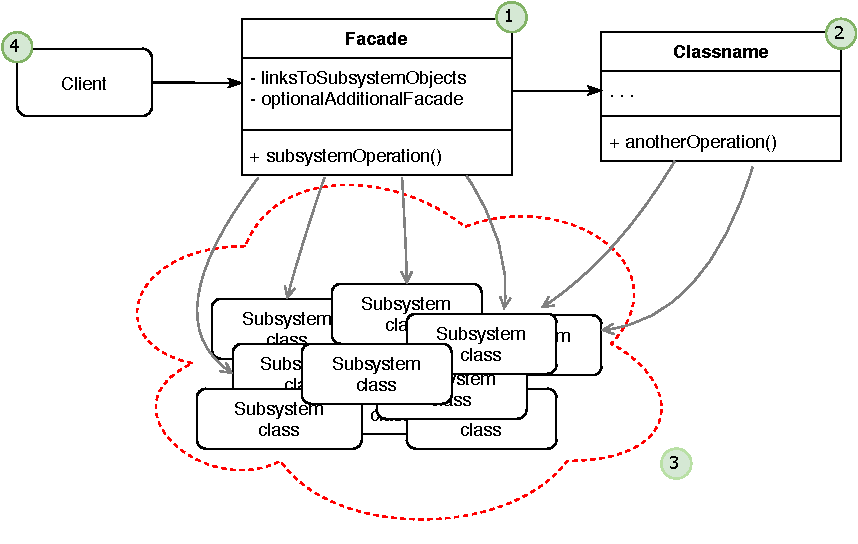
\includegraphics[width=0.75\textwidth]{images/03_1_facade_pattern.pdf}
    \caption{Componenti del Façade Pattern}
    \label{fig:facadepattern}
\end{figure}

\begin{enumerate}
    \item \textbf{Facade}: oggetto che dà accesso al set ristretto di funzionalità del Complex Subsystem
    \item \textbf{Additional Facade}: Facade aggiuntiva nel caso in cui si voglia tenere quella principale il più pulita e semplice possibile
    \item \textbf{Complex Subsytem}: libreria o framework complesso che vogliamo semplificare
    \item \textbf{Client}: Il client fa uso del Complex Subsystem attraverso la Facade
\end{enumerate}

%%%%%%%%%%%%%%%%%%%%%%%%%%%%%%%%%%%%%%%%%%%%%%%%%%%%%%%%%%%%%%%%%%%%%%%%%
\section{Documentazione}
La documentazione è stato il vero primo passo nel percorso di implementazione. Una decisione inusuale per lo sviluppo di un software, ma comprensibile per un caso di refactoring come questo, privo di una documentazione iniziale. 

%Sono state individuate un totale di 9 API da riscrivere, tutte originariamente sviluppate come metodi \emph{GET}. Di queste, 3 appartengono all'authentication server, mentre le restanti al booking server. Parte di queste API oltre alle operazioni sul database comprendono un sistema di notifica utente. Per queste API si è deciso di separare le due operazioni, delegando il sistema di notifica al \emph{Communication Server}.

\subsection{Swagger}
Swagger è un \emph{tool} composto da un set di software open source per progettare, creare e documentare \emph{RESTful APIs} attraverso l’\emph{OpenAPI Specification}, un formato di descrizione apposito per le REST APIs. In particolare aiuta a descrivere:

%%%%%%%%%%%%%%%%%%%%%%%%%%%%%%%%%%%%%%%%%%%%%%%%%%%%%%%%%%%%%%%%%%%%%%%%%

%%%%%%%%%%%%%%%%%%%%%%%%%%%%%%%%%%%%%%%%%%%%%%%%%%%%%%%%%%%%%%%%%%%%%%%%%

%%%%%%%%%%%%%%%%%%%%%%%%%%%%%%%%%%%%%%%%%%%%%%%%%%%%%%%%%%%%%%%%%%%%%%%%%

%%%%%%%%%%%%%%%%%%%%%%%%%%%%%%%%%%%%%%%%%%%%%%%%%%%%%%%%%%%%%%%%%%%%%%%%%

%%%%%%%%%%%%%%%%%%%%%%%%%%%%%%%%%%%%%%%%%%%%%%%%%%%%%%%%%%%%%%%%%%%%%%%%%